\documentclass[twoside,11pt]{article}

% Any additional packages needed should be included after jmlr2e.
% Note that jmlr2e.sty includes epsfig, amssymb, natbib and graphicx,
% and defines many common macros, such as 'proof' and 'example'.
%
% It also sets the bibliographystyle to plainnat; for more information on
% natbib citation styles, see the natbib documentation, a copy of which
% is archived at http://www.jmlr.org/format/natbib.pdf

\usepackage{jmlr2e}
\usepackage[ruled,vlined]{algorithm2e}

% Definitions of handy macros can go here

\newcommand{\dataset}{{\cal D}}
\newcommand{\fracpartial}[2]{\frac{\partial #1}{\partial  #2}}

% Heading arguments are {volume}{year}{pages}{date submitted}{date published}{paper id}{author-full-names}

%\jmlrheading{1}{2000}{1-48}{4/00}{10/00}{meila00a}{Marina Meil\u{a} and Michael I. Jordan}

% Short headings should be running head and authors last names

\ShortHeadings{Machine Learnable Image Compression Using Convolutional Autoencoders}{Fornia}
\firstpageno{1}

\begin{document}

\title{Machine Learnable Image Compression Using Convolutional Autoencoders}

\author{\name R. Paul Fornia \email paulfornia@gmail.com \\
       \addr Department of Computer Science\\
       Johns Hopkins University\\
       Baltimore, MD, USA
       %\AND
       %\name bob...\\
       }

%\editor{Kevin Murphy and Bernhard Sch{\"o}lkopf}

\maketitle

\begin{abstract}%   <- trailing '%' for backward compatibility of .sty file
I am seeking a practical image compression framework that performs well as both 
a) a traditional file compression and b) a feature set for which image 
classification can be performed with high accuracy. If successful, this would 
allow for highly accurate image classification to be applied directly to compressed 
images and may speed up training and fitting of image classifiers. I 
begin with a simplified version of the Compressive Autoencoder (AE) (CAE), 
which has already demonstrated 
promise as an image compression system, but which has not been tested directly 
in classification. I also propose a \emph{context-specialized} image compression, in
which an AE (such as a CAE) is used to initialize a classification problem, the 
labels are used to fine-tune the Deep Convolutional Neural Network (DNN)
 (as has been discussed in the classification
literature), a middle layer is quantized and taken as the compression, and new 
layers are trained on the compression (using the original image as the output) 
to turn it back into an effective AE.
\end{abstract}

\begin{keywords}
    Autoencoder, Compression, Convolutional Neural Network, Image Classification
\end{keywords}




\section{Background and Literature}

\subsection{Image Classification in Practice and Motivation}
The use of images in data pipelines is extremely common across industries and 
domains. Many of these applications include both image file compression and 
image classification steps. But many modern pipelines approach these as two 
separate problems – often first ingesting and compressing
images for storage, and then when needed for classification 
(training or fitting), they must be uncompressed back into a lossy version, 
similar to their original human-readable form.

 For instance, Facebook has published details of both compression and their 
facial recognition algorithm, and there is no indication that the two systems 
are integrated \citep{collet2016zstandard, taigman2014deepface}.

\subsection{Existing Efforts}

As several authors have noted, 
there would be considerable value in being able to perform machine learning 
tasks directly on the compressed images. \citet{needell2017} has written a classification 
algorithm that can be performed on any general binary file structure (including 
state-of-the art image compression methods), but this approach has not yet shown
 competitive classification performance. 

Conversely, \citet{fu2016} showed strong 
classification performance, but on cosine distance, which is not a competitive 
compression algorithm. The same can be said for any approach that performs 
embeddings or feature extraction, which can be viewed as a form of compression 
designed specifically for one ML task.

This paper will attempt to find one or more balanced methods that perform close 
to state-of-the-art as compression methods, and for which the compressed images 
can be classified without the need for decompression, with close to 
state-of-the-art at out-of-sample classification accuracy.

The most obvious starting point is the AE, which was originally 
devised as a compression algorithm, and has also inspired many elements of 
deep learning, which is the backbone of virtually all competitive image 
classification algorithms today.
AEs have many practical applications outside of compression, including 
pretraining deep neural networks, feature extraction, 
and image de-noising \citep{baldi2012autoencoders}. While some authors have claimed that AEs do 
not have practical value as compression algorithms
\footnote{
Multiple practical guides make this claim. For instance, \citet{huben2018_tds_ae} states ``autoencoders will 
do a poor job for [out-of-sample] image compression... JPEG will do vastly better.''
}
, recent work by 
\citet{theis2017} proposes a compressive, convolution autoencoder (CAE) that 
has shown great promise as an effective, practical image compression method, 
competitive with the JPEG file format.

\subsection{Contributions}

This paper will explore the effectiveness of the CAE as a “balanced” image compression standard, namely, one that a) is competitive among other compression algorithms on metrics such as loss, compression speed, and storage size, and b) can be used directly as a machine learning feature set in a way 
that provides competitive classification rates. Since AEs have already been explored at length as both compressors and as feature engineering methods, the first contribution of this paper is modest, and will simply “connect-the-dots” by finding one AE that works well at both tasks. 
To the best of my knowledge, this simple step does not appear in the literature as of early 2019.

Specifically, I will more thoroughly test the use of the CAE’s bottleneck layer as a fixed feature set in image classification. This can also be interpreted as using the AE to “pretrain” a DNN, but with fixed weights in the ``left" half\footnote{I will refer to NNs as running left-to-right, moving from the input data to the labeled data} of the network, and not allowing these initial weights to be “fine-tuned”. 
This idea is not inherently novel, and has been shown to be effective \citep{bengio2006pretrain}, but has not been shown using an AE that simultaneously performs well as a compression algorithm. I refer to this as a general image compression, because it is completely unsupervised, and does not rely on labels other than the image itself.

Finally, I propose a \emph{context-specialized} image compression. This version does allow weights to be fine-tuned to fit the labeled data, but then fixes the initial layers and trains a new set of layers to convert it back into the original image, thus making an effective AE. In contrast to the CAE, this method has been widely studied as a classifier (and achieves state-of-the art accuracy), but has not been fully explored as a compression technique.








\section{Fixed Transfers} \label{fixed}

The intended compression framework produces three components to its architecture, which are
 illustrated in Figure \ref{fig:three_stages}:
\begin{enumerate}
    \item Compression layers, which is similar to the ``left half" of an AE. 
    \item Decompression layers, which is similar to the “right half” of an AE. 
    \item Classification layers, which can be interpreted as either the right half of
     an end-to-end DNN classifier, or as the entire classifier trained on extracted (compressed) features. This portion can easily and quickly be retrained for each new classification problem.
\end{enumerate}

Both the general and specialized versions of the framework will output these three components.

\begin{figure}
  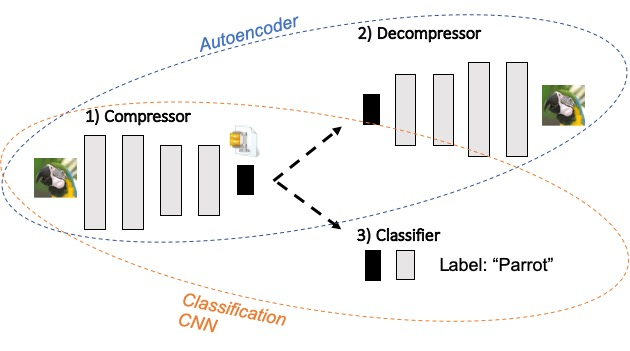
\includegraphics[width=\linewidth]{figures/three_stages.jpg}
  \caption{The three-stage machine learnable compression framework contains a compressor, a decompressor, and a classifier. Stages 1 and 2 together make an AE, stages 1 and 3 together make a DNN classifier. This paper considers the sharing of the compressor between both tasks. }
  \label{fig:three_stages}
\end{figure}

\subsection{General Compression training technique} \label{general}

For the general compression technique, I first replicate the CAE approach in order 
to get the best possible compression on the MNIST data (components 1 and 2). 
I then take the resulting compressed data (i.e., the bottleneck layer) and attempt 
to replicate high-performing classification DNN methods from the literature on 
the compressed data to predict the MNIST labels to create the classifier (component 3).
This process is illustrated in Figure \ref{fig:general}.

\begin{figure}
  \includegraphics[width=\linewidth]{figures/general.jpg}
  \caption{The “General Compression” framework. Blue layers are trained as AEs. Green layers are trained as DNN classifiers.}
  \label{fig:general}
\end{figure}

I will test the hypothesis that this classifier will perform on compressed data nearly as well as state-of-the-art classifiers on full-sized images. As the compressors did not utilize the labels, this hypothesis could be tested on any labeling domain, such as facial recognition, object recognition, or digit classification.

\subsection{Specialized Compression training technique} \label{special}

Using an AE as an initializer, I will replicate a high-performing DNN classifier
 from the literature. I will then select one of the hidden layers, and apply 
quantization techniques similar to those described in \citet{hubara2018}. This hidden layer 
will act as the compressed image. This DNN will make up components 1 and 3. I 
will then use the original image to train a new decompression layer (component 2).  
This is illustrated in Figure \ref{fig:specialized}.

\begin{figure}
  \includegraphics[width=\linewidth]{figures/specialized.jpg}
  \caption{The “Specialized Compression” framework.}
  \label{fig:specialized}
\end{figure}

Since components 1 and 2 are effectively built off standard DNN classifiers, 
this model’s efficacy as a classifier has already been shown at length in the 
literature \citep{krizhevsky2012imagenet}. I will reproduce this finding to support 
any tweaks to the compressed layer, such as quantization. I will then test the 
hypothesis that the decompressor performs similarly to other image compression methods.

\subsection{Extension of Specialized Compression training to other domains}

As time allows, and if the specialized compression proves effective, I will test 
how well it generalizes to other domains. For example, if a specialized compression 
framework is developed for facial recognition, I will apply the same compression 
to digits, retrain component 3) on the digit labels, and measure performance. 
This is closely related to the topic of transfer learning in DNNs \citep{yosinski2014}, 
but in order to preserve the functionality of the decompressor, does not allow for 
early layer fine-tuning.
This architecture is shown in Figure \ref{fig:ext_specialized}.

\begin{figure}
  \includegraphics[width=\linewidth]{figures/ext_specialized.jpg}
  \caption{The extension of the Specialized Compression framework to a new domain.}
  \label{fig:ext_specialized}
\end{figure}

I first test the hypothesis that images from another domain will still compress well. 
I expect that compression performance will be similar to that of the in-domain 
specialized compression. This prediction presumes that labels do not provide 
valuable compression information to the image.

I further hypothesize that this will underperform the specialized classification 
accuracy that was compressed using the correct domain. 
In other words, a state-of-the-art MNIST classifier will outperform a DNN in which 
early layers are trained for a different classification problem. 
This is almost certain to be the case. However, an interesting finding would arise 
if the difference is practically small, since a practitioner could then use 
a specialized compression optimized for their most common problem, knowing that 
they could still perform moderately accuracy classification in other contexts. 
For example, Facebook could optimize their compression for facial recognition, 
but could still perform some other ad hoc image recognition tasks from 
time-to-time with near optimal performance. This finding would be equivalent 
to stating that “fine tuning” the first layers adds little value in transfer learning of DNNs.







\section{Alternating Domain Training}

Ultimately, I will show that simply transfering the lower layers from one context to another 
does not provide comparable performance. Thus, the compression obtained by an AE
is not an effective feature set for classification, and the lower levels of a classifer 
CNN is not an effective compression technique. More on these finding are in 
Section \ref{results} below.

Having shown that an AE or CNN alone does not produce a general-purpose compression,
the question still remains on whether any such compression exists. 
The idea presented in this section is simple: continuously transfer the shared
initial layers between different contexts until results converge. 

The proposed algorithm is as follows:

\begin{enumerate}
\item{Train an AE for $k_{AE}$ epochs}
\item{Transfer the \emph{fixed} initial layers to a classifier, and train for 
$j$ epochs, as in Section \ref{fixed}.}
\item{Train the Classifier CNN for $k_{Class}$ epochs}
\end{enumerate}

\begin{algorithm}[H]
\SetAlgoLined
\KwResult{Compression, Decompression, and Classification NN components}
 Initialize model parameters for compression, decompression and classification layers
 \While{Either Classifier or AE Performance is improving}{
  %\eIf{condition}{
  % instructions1\;
  % instructions2\;
  % }{
  % instructions3\;
  %}
  Train entire AE (compressor and decompressor) for $k_{AE}$ epochs\;

  Train only Classifier layers for $j$ epochs, as in Section \ref{fixed}\;

  Measure Classification performance\;

  Train entire Classification CNN (compressor and classifier) for $k_{Class}$ epochs\;

  Train only Decompressor layers for $j$ epochs\;

  Measure AE performance\;
 }
 \caption{Alternating Target Training (one domain)}
\end{algorithm}









\section{Experiments and Results}


\subsection{Datasets}

I use three datasets in this paper:

\begin{enumerate}
\item{MNIST: Handwritten digits 0-9}
\item{KMNIST: Examples of ten handwritten Korean characters}
\item{Fashion-MNIST: Images of ten categories of clothing or accessories}
\end{enumerate}

These datasets are all greyscale, all 28x28 pixels, and all consist of ten classes.
In fact, KMNIST and Fashion-MNIST were created as easy ``drop-in'' replacements for MNIST.
A future direction of research could be to test color images and images of varying sizes.
Using images from different domains can provide a starting point for trasfering 
compression representations, even if the structure of the images from the different 
domains is very similar.

\subsection{Performance Metrics}

As all three datasets contain ten well-balanced classes, I simply use accuracy to measure
effectiveness of classification. 

\begin{equation}
Acc = \frac{Correct\ Predictions}{Total\ Predictions}
\end{equation}

For the AE, I measure performance by Peak Signal to Noise Ratio (PSNR), 
a conversion of Mean Squared Error (MSE) into the decibel scale, which is a common
performance metric of reconstructing lossy image compressions.

\begin{equation}
PSNR = 10*log_{10}\left(\frac{MAX^2_I}{MSE}\right)
\end{equation}

Where $MAX_I$ is the maximum pixel value, e.g. 255.


\subsection{Architecture}

For this paper, I propose an architecture for experimental purposes.
There is one primary limitation of the architecture as shown in Figure \ref{fig:three_stages}:
the initial layers of the AE must match the beginning of the classification architecture.
Here, ``initial layers of the AE'' mean all layers from the input to the bottleneck layer (inclusive).

I do not claim that the proposed architecture is the optimal one for this problem,
however, the architecture is loosely based on existing well performing networks, and so 
results are still strong enough for many practical applications.
Future research could focus on improvements to this architecture.

I begin with the well-known but simple LeNet-5 architecture %\cite{}
, with a small modification to account for the size of the MNIST data.
I also add dropout layers in the fully connected portion of the graph. 
This powerful addition helps prevent overfitting, and was popularized long
after the publication of LeNet-5. %\cite{}

The LeNet architecture also has another valuable property: a good bottleneck layer.
The last convolutional layer of LeNet contains about half the parameters of the input,
similar to many AE architectures. 

To create the Decompression layers, I simply work backwards from the compression layers of LeNet,
using similar convolutions, and upsample layers in place of maxpool layers.

Finally, I add a quantization to the bottleneck layer by rounding output values. %\cite{}
The input values of the datasets contain 28x28 pixels of integer values between 1 and 255.
The uncompressed image therefore can be represented by $28*28*log2(256) = 6272 = 784$ bytes.
The bottleneck layers contains 16 5x5 filters. 
After rounding the compressed values, outputs were integers between 0 and 15,
allowing compressed images to be stored in just $16*5*5*log2(16) = 1600 = 200$ bytes,
for a compression ratio of 25.5\%. 

%%Table of architecture here%%

\subsection{Baseline AE and Classifier}

While the architecture above is based on a classifier with good performance,
the architecture (especially the AE) is not necessarily state-of-the art. 
So in order to measure performance, I first run 50 epochs of both the full AE and Classifier,
both with randomly initialized parameters, allowing for the full network to be trained,
just as a traditional DNN would be. I measure performance on the test dataset as training progresses,
and find that improvement has leveled off by the 50th epoch.
This provides a good best-case-scenario benchmark for performance of the AE and Classifier. 

%%%Table of Baseline findings%%%%
\begin{table}
  \centering
  \includegraphics[]{figures/table_baseline.jpg}
  \caption{Baseline performance metrics of the full AE and Classification CNN. 
   Measured on an out-of-sample test dataset after 50 epochs of training.}
  \label{table:base}
\end{table}

%\begin{table}
%  \centering
%  \begin{tabular}{|c||c|c|}
    %\hline
    %\multicolumn{3}{|c|}{Baseline (50 Epochs of Training)}
    %\hline
    %Dataset & Classification Accuracy & Decompression PSNR \\
    %\hline
%  \end{tabular}
%  \caption{Baseline performance metrics of the full AE and Classification CNN. 
%   Measured on an out-of-sample test dataset after 50 epochs of training.}
%  \label{table:base2}
%\end{table}

\subsection{General Compression Experiment}

As described in section \ref{general}, I start with the baseline AE.
Using the lower layers, I compress all the images. This in effect ``freezes'' the 
lower layer parameters, and does not allow them to be fine tuned. 
I then train only the classifier layers on the compressed image.

%%%Insert Findings here%%%

I find that for all three datasets, the classification accuracy on the compressed images
is reasonably high (possibly good enough for some applications), but significantly 
short of the baseline.


\subsection{Specialized Compression}

As described in section \ref{special}, I start with the CNN that is trained by classification.
As above, I use the lower layers of this network to compress the image, then I train
only the decompressor layers on the compressed images, with the original images
as the target values.

%%Insert table%%

Just as with the general compression attempt, I find a AE with some value, but with 
significantly worse performance than the AE that is trained from the original images.


\subsection{Extension to Other Domain}

\subsection{Run-Time}




\section{Results} \label{results}


\subsection{Baseline}










\section{Possible Outcomes}

First, let us consider the worst-case scenario in the search for a balanced 
compression approach: it is possible that none of the above methods are 
effective at both tasks of learning and compression simultaneously. 
While the literature has found effective AEs at both tasks, it is possible that 
there is no such overlapping AE. 
It is possible that the AEs which have been shown to be good 
compressors/decompressors make lousy features, and that the AEs that are 
powerful feature extractors have practical problems as actual image 
compressors, either because compression/decompression is too slow, the 
compressed file is too large, or the reconstructed image is too lossy. 

If this is the case, I will further explore the literature on information theory, 
and attempt to explain this lack of overlap. I will explore whether this is 
an inevitable characteristic of the problem, 
or whether such a balanced approach may be possible in theory, and I have
simply failed to find one. 

If I succeed in finding an effective “balanced” AE as I hope, it could be either the general or specialized version (or both). 
If the general AE (which has already demonstrated value as a compression) is shown to be an effective feature set with near state-of-the-art classification accuracy, this would have substantial implications. 
In short, this would indicate that tuning the left-most layers of a DNN is unnecessary for all but the most accuracy-sensitive applications. If the specialized AE (already known to be an effective classifier) can be shown to be “recompressed” by training AE-style layers to the right of a classifier’s hidden layer, this could allow a path for practitioners to optimize their compression algorithms for specific common tasks. For example, a law enforcement agency could compress all their images in a way that is optimized for facial recognition with no loss in classification accuracy, and still be able to decompress back into human-readable images, nearly indistinguishable from any more traditional lossy image compression technique.








\section{Next Steps}

As time allows, I would like to explore the effects on compression, decompression, train, and fit computational performance. I expect that the train and fit steps will be faster than more traditional approaches, since fewer layers are involved. In particular, I am interested to explore how much time and memory is saved by not having to back-propagate or feed-forward through the left half of the layers. Comparisons of compression and decompression will require further research into existing compression methods and literature.

For all of the above analysis, I will begin with grey-scale, square images that have been normalized to the same size. As time allows, I will explore:
\begin{itemize}
    \item Extending the approach to color images
    \item Generalizing to images of varying sizes. Especially with the section on 
        Extension of the Specialized Compression, it would be useful to be able to 
        extend an autoencoder trained on images of one size to another domain, where 
        images may have a slightly different shape
    \item Speeding up the compression techniques by implementing and testing 
        the quantization NN techniques described in \citet{hubara2018}
\end{itemize}


Even if I succeed in finding a balanced, machine learnable compression, there are at 
least two substantial limitations (beyond those next steps listed above) that need 
to be addressed before such a compression will be a practical tool. These will most 
likely remain beyond the scope of this paper:
\begin{itemize}
    \item Despite the seemingly clumsy step of compressing/decompressing files, 
    such compressions have been highly optimized and are very fast. If the time saved 
    by this balanced, AE-based approach is too trivial, it may not be worth migrating
    to a lesser-known compression algorthm that could have compatibility issues.

    \item In many modern classification problems, there are valuable image 
    preprocessing steps performed prior to the machine learning. 
    For instance, Facebook first detects, aligns, and flattens its
    face representation before classifying them. This problem does not exist to the
    same extent in the
    standardized data used in this paper, but would need to be considered for most
    real-world applications.
\end{itemize}

%  blah blah sample citation ~\citep{pearl:88}.  Whether in their guise as 
%random fields), \emph{probabilistic graphical models} have a number 
%of uncertainty...\\

%{\noindent \em Remainder omitted in this sample. See http://www.jmlr.org/papers/ for full paper.}

% Acknowledgements should go at the end, before appendices and references

%\acks{We would like to acknowledge support for this project
%from the National Science Foundation (NSF grant IIS-9988642)
%and the Multidisciplinary Research Program of the Department
%of Defense (MURI N00014-00-1-0637). }

% Manual newpage inserted to improve layout of sample file - not
% needed in general before appendices/bibliography.

%\newpage

%\appendix
%\section*{Appendix A.}
%\label{app:theorem}

% Note: in this sample, the section number is hard-coded in. Following
% proper LaTeX conventions, it should properly be coded as a reference:

%In this appendix we prove the following theorem from
%Section~\ref{sec:textree-generalization}:

%\noindent
%{\bf Theorem} {\it Let $u,v,w$ be discrete variables such that $v, w$ do
%not co-occur with $u$ (i.e., $u\neq0\;\Rightarrow \;v=w=0$ in a given
%dataset $\dataset$). Let $N_{v0},N_{w0}$ be the number of data points for
%which $v=0, w=0$ respectively, and let $I_{uv},I_{uw}$ be the
%respective empirical mutual information values based on the sample
%$\dataset$. Then
%\[
%	N_{v0} \;>\; N_{w0}\;\;\Rightarrow\;\;I_{uv} \;\leq\;I_{uw}
%\]
%with equality only if $u$ is identically 0.} \hfill\BlackBox

%\noindent
%{\bf Proof}. We use the notation:
%\[
%P_v(i) \;=\;\frac{N_v^i}{N},\;\;\;i \neq 0;\;\;\;
%P_{v0}\;\equiv\;P_v(0)\; = \;1 - \sum_{i\neq 0}P_v(i).
%\]
%These values represent the (empirical) probabilities of $v$
%taking value $i\neq 0$ and 0 respectively.  Entropies will be denoted
%by $H$. We aim to show that $\fracpartial{I_{uv}}{P_{v0}} < 0$....\\

{%\noindent \em Remainder omitted in this sample. See http://www.jmlr.org/papers/ for full paper.}


\vskip 0.2in
%\bibliographystyle{unsrt}
\bibliography{paper}

\end{document}
